\documentclass[10pt,letterpaper]{report}
\usepackage[utf8]{inputenc}
\usepackage{amsmath}
\usepackage{amsfonts}
\usepackage{amssymb}
\usepackage{graphicx}
\usepackage{amsthm}
\usepackage[usenames, dvipsnames]{color}
\usepackage{textcomp}
\usepackage{mathtools}
\usepackage[left=2cm,right=2cm,top=2cm,bottom=2cm]{geometry}
\author{Brandon Caudell}
\title{Combinatorics of Rubik's Cubes}
\DeclarePairedDelimiter\ceil{\lceil}{\rceil}
\DeclarePairedDelimiter\floor{\lfloor}{\rfloor}
\definecolor{darkgreen}{RGB}{0, 128, 0}
\newtheorem{lemma}{Lemma}
\begin{document}
\maketitle
\newpage 
\tableofcontents
\newpage 
\chapter{Introductory Information}
\section{Origins of the Rubik's Cube}
\section{Basic Terminology}
The standard 3x3 Rubik's Cube has six colors, one for each face.  The typical color scheme is white, yellow, red, orange, green, and blue.  The cube contains 26 external pieces, known as \textbf{cubies} or simply pieces.  These cubies come in 3 variants: \textbf{centers}, \textbf{edges}, and \textbf{corners}.  Center cubies contain only one colored sticker, edge pieces contain two stickers, and corner cubies contain three stickers.\\

Each of the cube's six faces can be independently rotated by multiples of 90\textdegree.  When held in a particular position, the six faces of the cube are generally regarded as front, back, left, right, up, and down.  These terms give rise to the standard move notation of F,B,L,R,U,D to denote clockwise rotations by 90\textdegree of each face.\\

These six moves are enough to scramble and solve the puzzle in any possible way, though it is convenient to define additional moves for clarity.  An apostrophe is used to denote a counter-clockwise move, so F' is a counter-clockwise rotation about the front face.  Adding a superscript 2 denotes performing a move twice, i.e. a 180\textdegree rotation, so $B^2$ is a 180\textdegree rotation of the back face.  This is regarded as a half-turn.  Note that by symmetry of the square faces, performing a clockwise move twice is equivalent to performing the counter-clockwise version twice, i.e. $L^2 \cong (L')^2$, so we just use the first notation.  Also note that repeating a clockwise-move (quarter-turn) three times is equivalent to a single counter-clockwise move, and vise versa.\\

Occasionally, it is useful to talk about \textbf{slice} moves.  These are moves obtained by rotating any of the three central "slices" of the cube.  In the standard 3x3 cube, these are denoted by lowercase variants of the same 6 letters, with apostrophes and exponents having the same meaning as before.  Note that if we talk about a slice relative to a particular face, that face still defines the direction of the rotation, but we actually rotate the cubies one layer "deeper" into the cube.  These slice moves are isomorphic at the cube level to performing two face turns on opposite faces, i.e. the slice move $r \cong R'L$ (rotating the right face counter-clockwise and the left face clockwise).  Although the two move sequences are isomorphic, they leave the cube as a whole oriented differently, hence why it is useful to define them even if they are rarely used in the 3x3 cube.  \\

We need to establish a convention in how to read these move sequences.  Since moves, in general, are not commutative, reading a sequence of moves such as $LFR$ from right-to-left or left-to-right changes the resulting cube.  While mathematically this sequence of moves is very similar to function composition, which is typically done right-to-left, it is easier for us to "read off" a move sequence left-to-right, so that is the convention that we will operate under.  In cases where a right-to-left order makes sense, we will formally declare that distinction. \\

Note that when applying face moves to a cube, the center cubies remain fixed.  The four edge and four corner pieces on a face will rotate around, but the centers always maintain the same orientation relative to each other.  This extends to slice moves as well (since slice moves can be attained by a composition of face turns), but note that in slice moves the centers may move on the cube as a whole.  Their relative orientations, however, always remain the same.  In the standard coloring, white is opposite yellow, red is opposite orange, blue is opposite green, and if white is held as the bottom face then blue is to the left of red.  Because of these fixed centers, when solving a cube, the solver always knows what color a face must end up.
\section{Larger Cubes}
Unsurprisingly, larger cubes present more options.  Not just in the number of permutations that can be obtained, but in the number of different cases one must handle when solving.  Thus, our notation and understanding must adapt to different cube sizes.  In this report, we denote the size of a cube as its \textbf{order}, i.e. an order-3 cube is the standard 3x3 one.  Note that larger cubes may have multiple center cubies, and they need not be at the centers of faces.  We still use this terminology, though. \\

For cubes of higher order, we gain additional move options.  Whereas on the standard cube, we only needed 6 moves to scramble and solve, we will need 3 more moves for each increase in order by 1.  A proof of this fact will be given later, but we will outline the notation here.  We still use capital letters to denote face moves, and these 6 moves will never change even as order increases.  As the size of the cube goes up, what will change is the number of distinct slice moves that can be performed.  For a cube of order $r$, there are $\floor{\frac{r}{2}}-1$ \textit{indecomposable} slice moves for each face.  By indecomposable, we mean moves not isomorphic to any other move sequences (so the slice moves in our 3x3 cube are decomposable and therefore less important).  For the standard cube, this gives that there are no indecomposable slice moves.  For the 4x4 cube (also known as the Rubik's Revenge), there is one slice move per face.\\

To denote which slice move we are talking about (as there may be many for large cubes), we use a subscript indexed from 1 to this $\floor{\frac{r}{2}}-1$.  In the case of the order-4 and 5 cubes, we may also use the lower-case letter variant as before, i.e. $r = R_1$.  Primes and powers still work as before.  While slightly clunky, this notation allows us to unambiguously denote which move is being performed. \\

One important consideration with larger cubes is the presence or absence of fixed centers.  As we showed, the 3x3 cube has center cubies that never change orientation.  This is true of all odd-order cubes, as the only moves that would move the centers at all can be decomposed into other moves that leave the centers untouched (possibly with a rotation of the cube as a whole in order to maintain directionality).  Even-order cubes, however, lose this nicety.  Since every move is unique and indecomposable, and there are multiple center cubies that will move independently of each other, it is up to the solver to ensure that the faces are actually reassembled in the correct relative orientations.  Not only must all colors be reassembled opposite their correct opposing color, but the relative orientations must be correct as well.  For instance, the white-red-blue corner piece is oriented such that the blue face should be left of red if the white face is pointed down.  If this orientation is not upheld, then the solve will not complete.
\chapter{Groups in the Rubik's Cube}
The first obvious question regarding the Rubik's Cube is ``How many possible scrambled states can the puzzle be in?''.  In order to answer this question, we need to understand the cube and its moves as an algebraic group.  We will start at a larger group and refine it down to our answer.
\section{The Sticker Group}
Given a cube of order $n$, it is easy to count the total number of stickers on it to be $6n^2$.  These stickers are partitioned into 6 different colors, one color per face on the solved cube.  Although clearly each sticker is ``locked'' to a cubie and thus the locations on the cube it can be moved to via legal moves are very limited, it is useful to think about what could happen if this constraint were removed. \\

If we were to take all the stickers off of the plastic cube body and rearrange them with no restrictions, then in how many ways could we do this?  If we assume each sticker is distinguishable (two red stickers can somehow be differentiated), then this sticker arrangement is just a permutation of $6n^2$ items.  We denote the algebraic group of these sticker rearrangements as the \textbf{Sticker Group of order n}.  The symbol we will use for this is $\mathcal{S}_n$.  This group is isomorphic to the symmetric group of order $6n^2$ for obvious reasons.  Thus, $\mathcal{S}_n \cong \mathfrak{S}_{6n^2}$. \\

Clearly, this is an extremely loose upper bound on the number of possible states of a valid Cube.  Let us go one level closer to the answer to our question.

\section{The (Re)assembly Group}
Permuting the stickers around is not really the group action we care about.  We would much rather consider actions on the cubies themselves, since those are the pieces being moved in legal rubiks moves.  Let us consider the group formed by arbitrarily taking the cube apart (leaving the stickers alone) and reassembling the cubies.  This group on a cube of order $n$ will be known as the \textbf{(Re)assembly group} of order $n$, denoted $\mathcal{A}_n$.  There will be a number of restrictions imposed on us by the physical nature of the cube, and we will account for these one at a time.

\subsection{Cubie Type Restrictions}

The reassembly group structure with the fewest restrictions will only respect the cubie types.  Corners must remain corners, etc.  Thus, we will consider the number of each cubie type and our freedom to position and orient them.  Note that the reassemblies of each cubie type are independent of each other, thus we can consider them independently and then form a direct product group. \\

Regardless of the cube size, there will always be exactly eight corner pieces.  These pieces can be freely permuted, and each one can be oriented in one of three orientations.  This relationship can be most aptly described as a wreath product \begin{align*}
C_3 \wr \mathfrak{S}_8
\end{align*}

A wreath product of the form $G \wr \mathfrak{S}_n$ can be thought of as an $n$ by $n$ matrix with exactly one non-zero element in each row and column, with those nonzero elements coming from $G$.  This is similar to a permutation matrix (stemming from the $\mathfrak{S}_n$ component), with the additional freedom that each element can be chosen from $G$.  This suits our needs as we are permutating the 8 corner cubies and orienting each in one of 3 cyclic orientations. \\

The edge cubies work similarly, but the number of each is a function of the cube size.  For a cube of size $n$, there will be 12 edge ``segments'' and $n-2$ cubies for each.  Each edge cubie can be oriented in one of two orientations.  Thus, our group structure for the edge assembly is \begin{align*}
C_2 \wr \mathfrak{S}_{12(n-2)}
\end{align*} \\

Finally, we consider the center cubies.  Here, we will actually impose one small further restriction.  For reasons that we will see later, we will only consider \textbf{odd} sized cubes, and we will not allow reassembly of the ``true-centers''.  We know that legal rubiks moves preserve the positions of these true-centers, so we can simplify our problem by not allowing them to be moved in the reassembly group.  The restriction to odd-sized cubes is thus needed because even-order cubes don't have true-centers. \\

Given a cube of odd size $n$, each of the six faces will have $(n-2)^2 -1$ center cubies, not counting the true centers.  Assuming all such centers are distinguishable, our center reassembly group has the form \begin{align*}
\mathfrak{S}_{6(n-2)^2 - 6}
\end{align*}

Thus, the group structure for this first version of the reassembly group is\begin{align*}
\mathcal{A}_n = (C_3 \wr \mathfrak{S}_8) \times (C_2 \wr \mathfrak{S}_{12(n-2)}) \times \mathfrak{S}_{6(n-2)^2 - 6}
\end{align*}

\subsection{Cubie Sub-Type Restrictions}
The next restriction to apply to this group involves so-called cubie ``sub-types''.  These don't exist on the standard order-3 cube, but cubes of order 5 and above have multiple sub-types of edge and center cubies.  The diagram below illustrates what I mean.

\begin{center}
\includegraphics[scale=.5]{images/professorsCubeLabelled.png} 
\end{center}

As with any sized cube, the corners of an order-5 cube can be freely permuted and oriented because they all have the same shape inside the cube.  The other two piece types, however, have different internal shapes depending on where exactly in the puzzle they go.  An edge cubie on the midpoint (labelled E1) will have a different shape than one labelled E2, etc.  Because of this, we now need to partition the edge and center cubie subgroups based on sub-types, as a reassembly cannot intermingle cubies of different sub-types.  Their different internal shapes prohibit that. \\

For the edges, the sub-types are determined by distance from the midpoint of the edge.  For an odd-order cube (which we have restricted ourselves to) there will be always be a sub-type of midpoint-edges containing 12 cubies total.  All other edge sub-types will contain 24 cubies.  The number of those edge sub-types for a cube of order $n$ is $\floor{\frac{n-2}{2}}$.  Thus, we decompose our edge reassembly subgroup from before down to \begin{align*}
(C_2 \wr \mathfrak{S}_{12}) \times \Big( \bigotimes_{i=1}^{\floor{\frac{n-2}{2}}} (C_2 \wr \mathfrak{S}_{24}) \Big)
&= (C_2 \wr \mathfrak{S}_{12}) \times \Big( \bigotimes_{i=1}^{\frac{n-3}{2}} (C_2 \wr \mathfrak{S}_{24}) \Big)
\end{align*}

where the $\bigotimes$ denotes repeated direct product.  The last step removes the floor operator by noting that $n$ is odd. \\

The center cubies will work similarly, albeit with a little more complexity in the number of sub-types.  Consider this matrix representing the centers of a face on an order-9 cube.  The labels are the center sub-type for each cubie.  Remember that we are ignoring the true-center (labelled by a 0) because reassemblies cannot premute them.
\begin{center}
\begin{tabular}{|c|c|c|c|c|c|c|}
\hline 
7 & 8 & 9 & 10 & 11 & 12 & 7 \\ 
\hline 
• & 3 & 4 & 5 & 6 & 3 & • \\ 
\hline 
• & • & 1 & 2 & 1 & • & • \\ 
\hline 
• & • & • & 0 & • & • & • \\ 
\hline 
• & • & • & • & • & • & • \\ 
\hline 
• & • & • & • & • & • & • \\ 
\hline 
• & • & • & • & • & • & • \\ 
\hline 
\end{tabular} 
\end{center}

Note that any cubies that lie on a diagonal from the true-center are partitioned into sub-types based on their diagonal-distance from the center.  All other cubies that lie in this labelled triangle lie in distinct sub-types.  It might be tempting to think that the cubies labelled 4 and 6 are in the same sub-type and could be swapped in a reassembly, but this turns out to not be the case.  The pieces themselves are mirror images of each other, and thus cannot be swapped in an assembly. \\

We now trim-down this diagram to ignore the true-centers, and to label only one representative from each of the ``diagonal'' sub-types.  We will also color the remaining labels to make counting easier soon.

\begin{center}
\begin{tabular}{|c|c|c|c|c|c|c|}
\hline 
• & \textcolor{red}{8} & \textcolor{red}{9} & \textcolor{blue}{10} & \textcolor{darkgreen}{11} & \textcolor{darkgreen}{12} & \textcolor{darkgreen}{7} \\ 
\hline 
• & • & \textcolor{red}{4} & \textcolor{blue}{5} & \textcolor{darkgreen}{6} & \textcolor{darkgreen}{3} & • \\ 
\hline 
• & • & • & \textcolor{blue}{2} & \textcolor{darkgreen}{1} & • & • \\ 
\hline 
• & • & • & • & • & • & • \\ 
\hline 
• & • & • & • & • & • & • \\ 
\hline 
• & • & • & • & • & • & • \\ 
\hline 
• & • & • & • & • & • & • \\ 
\hline 
\end{tabular} 
\end{center}

This matrix now contains exactly one representative from every center sub-type for this order-9 cube.  To verify this, imagine rotating the matrix by 90 degrees three times.  Each entry in the matrix (except for the true-center) will be assigned a label exactly once, thus a valid partition will emerge.  Note that the partitions will all be equally-sized (4 cubies per face per sub-type).  Thus, we need only to derive a formula for counting the number of sub-types for an arbitrarily-sized cube. \\

The coloring makes a counting system rather straightforward.  For a cube of size $n$ (still assuming odd), there will be $\sum_{i=1}^{\floor{\frac{n-4}{2}}}i$ elements in the red triangle.  Remember that the above matrix was formed from a cube of order 9, not 7.  The blue strip will contain $\floor{\frac{n-2}{2}}$ cubies.  Finally, the green triangle will contain $\sum_{i=1}^{\floor{\frac{n-2}{2}}}i$ cubies.  Using summation formulas and adding these up yields the number of center sub-types for a cube of order $n$ as \begin{align*}
\sum_{i=1}^{\floor{\frac{n-4}{2}}}i + \floor{\frac{n-2}{2}} + \sum_{i=1}^{\floor{\frac{n-2}{2}}}i
&= \frac{\Big(\floor{\frac{n-4}{2}}\Big)\Big(\floor{\frac{n-4}{2}} + 1\Big)}{2} 
+ \floor{\frac{n-2}{2}} + 
\frac{\Big(\floor{\frac{n-2}{2}}\Big)\Big(\floor{\frac{n-2}{2}} + 1\Big)}{2} \\
&=\frac{\Big(\frac{n-5}{2}\Big)\Big(\frac{n-5}{2} + 1\Big)}{2} 
+ \frac{n-3}{2} + 
\frac{\Big(\frac{n-3}{2}\Big)\Big(\frac{n-3}{2} + 1\Big)}{2} \\
&= \frac{\frac{(n-5)^2}{4} + \frac{n-5}{2} + n - 3 + \frac{(n-3)^2}{4} + \frac{n-3}{2}}{2} \\
&= \frac{(n-5)^2 + 2(n-5) + 4(n-3) + (n-3)^2 + 2(n-3)}{8} \\
&= \frac{n^2 - 10n + 25 + 2n - 10 + 4n - 12 + n^2 - 6n + 9 + 2n - 6}{8} \\
&= \frac{2n^2 - 8n + 6}{8} \\
&= \frac{n^2 - 4n + 3}{4} \\
&= \frac{(n-3)(n-1)}{4}
\end{align*}

It is worth providing a quick justification that this value will always be an integer.  For $n=3$ there are no center sub-types (as we are disregarding the true-centers), and our formula yields 0.  For any odd number $n \geq 5$, consider the values of $n-3,n-1$.  These will be consecutive even numbers.  As such, one of them must be divisible by 4.  From this, we know that the formula presented above will always yield an integer value for odd $n \geq 5$. \\

As we've shown, each center sub-type formed in this way will contain exactly 24 cubies (four per face).  Thus, we can write our center reassembly subgroup with this constraint as

\begin{align*}
\bigotimes_{i=1}^{\frac{(n-3)(n-1)}{4}}\mathfrak{S}_{24}
\end{align*}

We can now write the reassembly group of order n as \begin{align*}
\mathcal{A}_n = (C_3 \wr \mathfrak{S}_8) \times (C_2 \wr \mathfrak{S}_{12}) \times \Big( \bigotimes_{i=1}^{\frac{n-3}{2}} (C_2 \wr \mathfrak{S}_{24}) \Big) \times \Big( \bigotimes_{i=1}^{\frac{(n-3)(n-1)}{4}}\mathfrak{S}_{24} \Big)
\end{align*}

\subsection{Edge Sub-Type Orientation Restriction}
The last observation to note has to do with the orientation of edge cubies.  For any edge cubie that is not at the midpoint of the edge, the piece structure actually limits the orientation it can be in.  Consider a pair of edge cubies adjacent to the midpoint of an order-5 cube, as shown here.

\begin{center}
\includegraphics[scale=.5]{images/professorsCubeMarked.png} 
\end{center}

The internal shapes of these pieces are actually mirror images of each other.  Thus, during a reassembly, one can swap the positions of these two.  However, the pieces are asymmetric, meaning that one cannot take the cubie marked with a blue arrow and flip its orientation in-place.  The internal shape of the piece will prevent that.  In fact, for any edge cubie other than one in the midpoint sub-type, the position it is in actually determines the orientation it must be in.  The edge cubie marked with a green arrow cannot change orientation in-place, nor can it be moved to the blue-arrow location while keeping the while sticker pointing forward.  The position wholly determines the orientation of these pieces. \\

This can be easily reflected in the group structure by removing the wreath product from the edge cubie sub-types (other than the midpoint sub-type).  This means that our final reassembly group of order n has the group structure

\begin{align*}
\mathcal{A}_n = (C_3 \wr \mathfrak{S}_8) \times (C_2 \wr \mathfrak{S}_{12}) \times \Big( \bigotimes_{i=1}^{\frac{n-3}{2}}\mathfrak{S}_{24} \Big) \times \Big( \bigotimes_{i=1}^{\frac{(n-3)(n-1)}{4}}\mathfrak{S}_{24} \Big)
\end{align*}

Broadly speaking, the first factor subgroup is the positions and orientations of the corner cubies.  The second is the positions and orientations of the \textit{midpoint} edge cubies.  The third is a sequence of subgroups relating to the positions of each non-midpoint edge sub-type.  Again, these positions wholly determine the orientations, which is why they are purely symmetric.  The final subgroup is the positions of each center sub-type (remember that the true-centers are ignored).  Orientation is not a factor in the center cubies, so position is the only concern. \\

It is important to note that these last two factors are not present in the $n=3$ case.  The standard cube has \textit{only} midpoint edges and \textit{only} true-centers.  Thus, $\mathcal{A}_3 = (C_3 \wr \mathfrak{S}_8) \times (C_2 \wr \mathfrak{S}_{12})$, which is the same as the formula we derived before we applied these restrictions.

\section{The Rubik Group}
Even without proof, it is not hard to imagine that not all reassemblies of a Cube are reachable by valid moves.  It is common knowledge amongst solvers that taking any one edge of a cube and swapping the stickers on it creates an unsolvable puzzle.  This alone tells us that not all the reassemblies of a cube are in the Rubik's Group, which is formally defined to be the group of configurations that can be reached via legal turns of the Cube.  Equally, this group can be defined as the configurations one can solve the cube from.  In either case, we denote the set of all such assemblies of a cube of order $n$ by the \textbf{Rubik Group}, $\mathcal{R}_n$.  Another way to view this group is the subgroup of the reassembly group generated by the six legal rubiks moves.  \\

Calculating the Rubik Group for arbitrarily-sized cubes is no small endeavor, so we will start with $\mathcal{R}_3$, the standard cube.  It is worth noting that the Assembly Group of order 3 contains about $5.19 \times 10^{20}$ elements, or 519 quintillion.  Quite a large number considering the small size of the standard cube.  So clearly, its Rubik Group will also contain a large number of elements.  Recall that \begin{align*}
\mathcal{A}_3 \cong (C_3 \wr \mathfrak{S}_8) \times (C_2 \wr \mathfrak{S}_{12})
\end{align*}

To calculate the size of the Rubik group, we will form a homomorphism $f : \mathcal{A}_3 \rightarrow G$ for some group $G$, the kernel of which will be $\mathcal{R}_3$.  This $G$ will be the direct product of three component groups $G_i, 1 \leq i \leq 3$.  For each $G_i$, there will be an associated homomorphism $f_i : \mathcal{A}_3 \rightarrow G_i$.  From these, we will make \begin{align*}
f(\sigma) = (f_1(\sigma), f_2(\sigma), f_3(\sigma))
\end{align*}
These $f_i$ will be provably orthogonal, meaning that the kernel of $f$ will be exactly the intersection of the kernels of the $f_i$.

\subsection{Cubie Positions}

The first subgroup $G_1$ will consider the positions (not orientations) of the edge and corner cubies.  We will first define two other homomorphisms to help us write a formal definition for $f_1$.  Let $g_e : \mathcal{A}_3 \rightarrow \mathfrak{S}_{12}$ represent the edge cubie permutation.  This will be a projection to the edge cubie component (there is only one in $\mathcal{A}_3$) that ignores the orientations of each.  This is well defined from how we defined the wreath product $C_2 \wr \mathfrak{S}_{12}$. \\

Similarly, we define $g_c : \mathcal{A}_3 \rightarrow \mathfrak{S}_{12}$ to be a projection based on the corner cubie positions.  Again, this will ignore the orientations of each and focus only on their permutation.  This is equally well-defined. \\

Now consider the homomorphism $p_n : \mathfrak{S}_n \rightarrow C_2$, defined as follows: \begin{align*}
p_n(\sigma) = \begin{cases}
1 & \sigma \in A_n \\
-1 & \sigma \notin A_n
\end{cases}
\end{align*}
where $A_n$ is the alternating subgroup of $\mathfrak{S}_n$.  This homomorphism denotes the \textbf{parity} of a permutation.  This value denotes whether it is an even- or odd-permutation, and will be of use to us.  We will quickly validate that this is, in fact, a homomorphism.  Let $\alpha, \beta \in \mathfrak{S}_n$ both be either even- or odd-permutations.  In either case, their composition $\alpha \beta \in A_n$, i.e. will have even permutation, and $p_n(\alpha) \cdot p_n(\beta) = 1$. \\

On the other hand, suppose that the permutations $\alpha, \beta$ have opposite parities.  WLOG, assume $p_n(\alpha) = 1, p_n(\beta) = -1$.  Then $p_n(\alpha) \cdot p_n(\beta) = 1 \cdot -1 = -1$, and the composition $\alpha \beta \notin A_n$, i.e. will be an odd permutation.  Thus, $p_n(\alpha \beta) = p_n(\alpha) p_n(\beta) = -1$.  In either case, the homomorphism requirement is satisfied. \\

With all this in mind, we can now write a definition for $f_1: \mathcal{A}_3 \rightarrow C_2$ as 
\begin{align*}
f_1(\sigma) = (p_8 \circ g_c(\sigma)) \cdot (p_{12} \circ g_e(\sigma))
\end{align*}
Verbally, this homomorphism can be thought of as being $1$ if the parities of both the edge and corner permutations are equal, and $-1$ if they are not equal.  This is a well-defined homomorphism because it is a composition and product of other well-defined homomorphisms. \\

The kernel of $f_1$ is the set $\{\sigma \in \mathcal{A}_3 : p_{12} \circ g_e(\sigma) = p_8 \circ g_c (\sigma) \}$.  I.e. the permutations of edge and corner cubies (irrespective of orientations) are either both even or both odd.  We will now show that $\mathcal{R}_3 \subseteq \text{ker}(f_1)$. \\

Clearly the solved state (which is the identity of $\mathcal{A}_3$ and $\mathcal{R}_3$) is in the kernel, because the identity is in the kernel of any homomorphism.  Now consider any of the six generators of $\mathcal{R}_3$, which are the six face turns on the cube.  The generators are equal up to isomorphism, so we can arbitrarily choose one.  We will look at the cycle structure of the cubie positions such a move induces.

\begin{center}
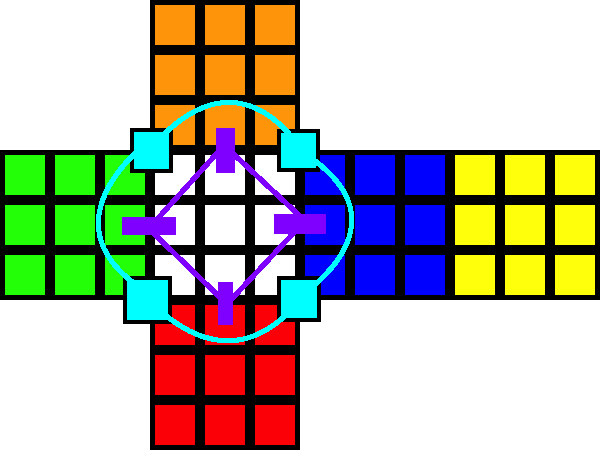
\includegraphics[scale=.5]{images/faceCubieCycle.png} 
\end{center}

In any face turn, we see exactly two four-cycles: one of the edge cubies and one of the corners.  Let $\alpha \in \mathcal{R}_3$ be such a move.  Because a four-cycle is an odd-permutation, applying it to any element of the symmetric group containing it will toggle the parity of that element.  As such, we see that $p_{8} \circ g_c (\alpha) = p_{12} \circ g_e (\alpha) = -1$.  Thus, $f_1(\alpha) = 1$ and $\alpha \in \text{ker}(f_1)$.  Thus, any face turn is in the kernel of $f_1$.  \\

Note that the kernel of a homomorphism is a normal subgroup, and therefore closed under group multiplication.  Because we have shown that any generator of $\mathcal{R}_3$ is an element of $\text{ker}(f_1)$, and any element of the group can be expressed as a product of generators (by definition), we have that $\mathcal{R}_3 \subseteq \text{ker}(f_1)$.

\subsection{Edge Orientations}

For our next homomorphism, $f_2$, we will focus on the orientations of the edge cubies.  We will derive a homomorphism $f_2 : \mathcal{A}_3 \rightarrow C_2$ that denotes the ``total'' orientation of all twelve edges.  \\

Formally, we first define $h: \mathcal{A}_3 \rightarrow C_2 \wr \mathfrak{S}_{12}$ be the projection map down to the edge cubie component of our reassembly group.  Let $g_i : C_2 \wr \mathfrak{S}_{12} \rightarrow C_2, 1 \leq i \leq 12$ be homomorphisms that look at the orientations of the 12 distinct edge cubies (arbitrarily ordered).  These can be thought of as reading off the value from $C_2$ that is the nonzero entry of the $i$th column in the matrix element of $C_2 \wr \mathfrak{S}_{12}$.  These are well-defined homomorphisms that just throw-away information in $\mathcal{A}_3$ that we aren't currently concerned with.  We can then define $f_2: \mathcal{A}_3 \rightarrow C_2$ by
\begin{align*}
f_2(\sigma) = \Pi_{i=1}^{12}g_i \circ h (\sigma)
\end{align*}  
I.e. taking the orientations of each of the twelve edges and forming their product.  We will prove this is a well-defined homomorphism using the following lemma.

\begin{lemma}
Let $G,H$ be groups, with $H$ abelian.  Let $f,g:G \rightarrow H$ be homomorphisms.  Then $k: G \rightarrow H$ defined by $k(x) = f(x)g(x)$ is a homomorphism.
\end{lemma}

\begin{proof}
Let $a,b \in G$.  Then,
\begin{align*}
k(ab) &= f(ab)g(ab) \\
&= f(a)f(b)g(a)g(b) \\
&= f(a)g(a)f(b)g(b) \\
&= k(a)k(b)
\end{align*}
\end{proof}

This same argument can be extended to apply to any number of homomorphisms, in our case the $g_i \circ h$'s.  Since $C_2$ is abelian, this theorem applies, and $f_2$ is a homomorphism. \\

Now, we will prove that $\mathcal{R}_3 \subseteq \text{ker}(f_2)$.  To do this, we need to prove that any solvable configuration of the cube has the ``total'' orientation of its edge cubies be positive.  We will show this is the case by proving that any face-turn of the cube will toggle the orientation of all four edge cubies involved in it.  Consider the set of all position-orientation pairs that a cubie can exist in.  There are twelve positions, each with two orientations.  We now form a graph with the vertex set being these 24 items, and the edge set being those pairs which can be reached via exactly one face turn from each other.  Such a graph looks like this.

\begin{center}
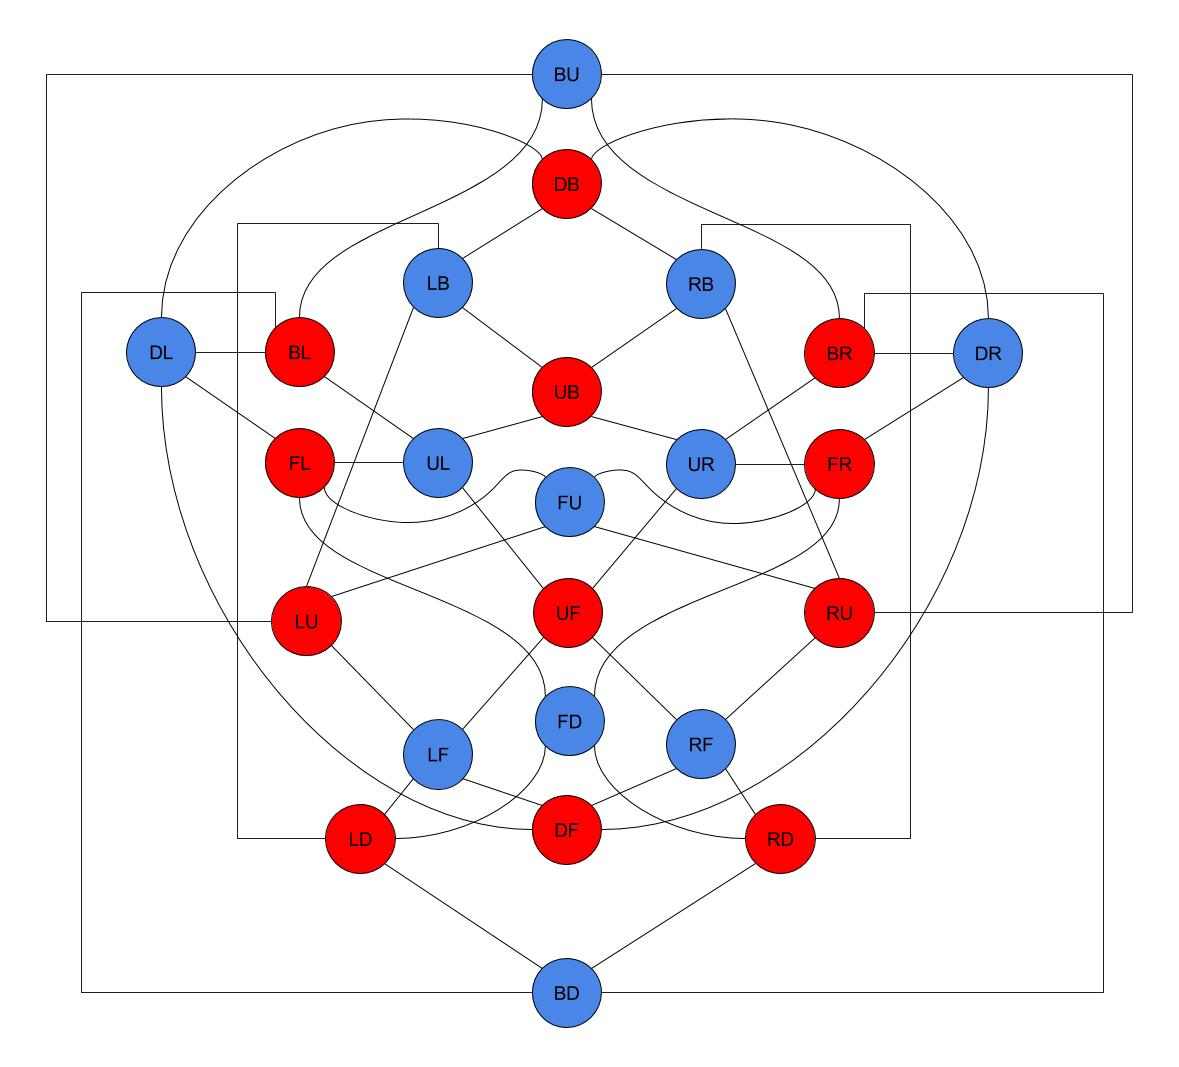
\includegraphics[scale=.35]{images/Rubiks_Edge_Graph.jpg} 
\end{center}

Note that this graph is bipartite, as indicated by the two-coloring.  Also note that for each position, its two orientations are in opposite partite sets.  I.e. $UR$ is blue, and $RU$ is red.  These facts mean that we can define a valid orientation scheme such that the orientation system is well-defined, and any time an edge cubie undergoes a face turn, its orientation flips.  Thus, when any face turn is applied, all four edge cubies affected flip orientation. \\

Since this happens to an even number of edge cubies in any face turn, the total orientation will be preserved.  In other words, if $\alpha$ is any face turn in $\mathcal{R}_3$, then $f_2(\alpha) = 1$ and $\alpha \in \text{ker}(f_2)$.  Just as with $f_1$, this shows that $\mathcal{R}_3 \subseteq \text{ker}(f_2)$ due to the face turns being generators for $\mathcal{R}_3$.

\subsection{Corner Orientations}

We will now prove a similar claim for the corner orientations.  We will define a homomorphism $f_3 : \mathcal{A}_3 \rightarrow C_3$ that denotes the total orientation of the corner cubies, and prove that $\mathcal{R}_3 \subseteq \text{ker}(f_3)$. \\

Just as before, let $h: \mathcal{A}_3 \rightarrow C_3 \wr \mathfrak{S}_8$ be the projection map to the corner cubie component.  Next, let $g_i: C_3 \wr \mathfrak{S}_8 \rightarrow C_3, 1 \leq i \leq 8$ be homomorphisms that look at the orientation for each of the 8 corner cubies.  Now we define $f_3$ by
\begin{align*}
f_3(\sigma) = \Pi_{i=1}^{8}g_i \circ h (\sigma)
\end{align*}

Again, because $C_3$ is abelian, this is a well-defined homomorphism.  We now must prove that any face turn preserves the total orientation of the corner cubies.  While there is probably a way to prove this property using a graph as well, the graph in question would be a 6-regular graph on 24 vertices, and it is not obvious what property we would even be looking for.  Because of this, we will fall back to a more brute-force approach.  \\

Consider an orientation scheme for the corners defined as follows.  Start with a solved cube, and label the stickers on each of the corner cubies $0,1,2$ in cyclic order, with the $0$ being placed on the white or yellow sticker and proceeding in clockwise order.  Every corner cubie has either a white or yellow sticker, so this is well-defined.  The resulting labelling looks as follows:

\begin{center}
\includegraphics[scale=1.5]{images/cornerOrientation.png} 
\end{center}

Note that these labelings are values in $\mathbb{Z}_3$ rather than $C_3$.  These groups are isomorphic, so we will introduce the simple isomorphism $q: \mathbb{Z}_3 \rightarrow C_3$, $q(0) = 1, q(1) = \omega, q(2) = \omega^2$ where $\omega$ is the primitive 3rd root of unity.  This will bridge the gap between these groups. \\

Now we may introduce a shortcut for each $g_i \circ h$.  For corner $i$ (which one may arbitrarily have ordered), read off the label on either the white or yellow face, and then apply the isomorphism $q$.  This is well-defined as every corner cubie must have exactly one sticker on exactly one of those faces. \\

Because all of these functions are homomorphic, we can carry this shortcut up to $f_3$.  For some cube configuration $\sigma$, $f_3(\sigma)$ will be the result of applying $q$ to the sum mod 3 of the labels on the white and yellow faces.  With this machinery in place, we can look at what happens to $f_3(\alpha \sigma)$ for different face turns $\alpha$.  Note that in this setup, not all face turns are identical, because the white and yellow faces have extra meaning. \\

If $\alpha$ were either the white or yellow face, then the result of $f_3(\alpha)$ is rather trivial.  In either case, the zeroes just rotates around the appropriate face, and the sum of labelings won't change.  Thus, $f_3(\alpha) = q(0) = 1$. \\

The more interesting cases are the other four face turns.  These four are all identical up to isomorphism.  In the solved state, each of these four faces all contains a pair of 1's and a pair of 2's, with each pair being diagonal from itself.  Thus, we can arbitrarily choose one face to rotate.  In choosing the red face, the result is as follows:

\begin{center}
\includegraphics[scale=1.5]{images/rotatedCornerOrientation.png} 
\end{center}

Note that in adding up the values on the white and yellow faces, the result is $6 \cong_3 0$.  In looking a little closer, we see why this is the case.  Consider the two corner cubie locations in the white face that were affected.  If we ignore the fact that specific cubies left and entered these locations and look solely at the change in orientation, we see that the two locations changed orientation in offsetting ways.  The front-up-left corner location had its cubie turned 120 degrees counter-clockwise (a change of $+1$).  The front-up-right corner cubie location experienced a clockwise rotation by the same amount (a change of $-1 \cong_3 +2$).  These two changes offset, causing the sum of the white face mod 3 to remain zero.  A similar scenario occurred on the yellow face: the corner orientation changes offset. \\

Since these corner-offsets will happen independent of the starting state of the cube, it is clear that any face-turn will preserve the orientation sum of the corners.  And since these face turns are the generators of $\mathcal{R}_3$, it is clear that $\mathcal{R}_3 \subseteq \text{ker}(f_3)$.

\subsection{Putting it all together}
Now, we have formed three homomorphisms $f_1,f_2,f_3$ and shown that $\mathcal{R}_3$ lies inside the kernel of each.  We now consider the homomorphism $f: \mathcal{A}_3 \rightarrow C_2 \times C_2 \times C_3$ formed by $f(\sigma) = (f_1(\sigma), f_2(\sigma), f_3(\sigma))$.  From what we have proven thus far, it is clear that $\mathcal{R}_3 \subseteq \text{ker}(f)$.  We will prove that, in fact, $\mathcal{R}_3 = \text{ker}(f)$.  In typical fashion, this set equality will be proven by showing that $\text{ker}(f) \subseteq \mathcal{R}_3$.  To do this, we will provide a number of legal move sequences that each perform a small operation on the cube state.  These operations can be sequenced to solve any cube state that lies in the kernel of $f$, showing the subset property desired. \\

Let $\sigma \in \text{ker}(f)$ be a cube assembly.  From what we have proven, we know three crucial, orthogonal facts about $\sigma$.  \begin{enumerate}
\item The parities of the permutations of the edge and corner cubies are equal.
\item The total orientation the edges is zero.
\item The total orientation of the corners is zero.
\end{enumerate}

\subsubsection{Positioning Edges}

The first move sequence we list will swap the positions of exactly two edge cubies.  It will also permute the corner cubies somewhat (as it must in order to preserve property 1), but this will not be a concern yet.  The move sequence is listed below, and is read from left to right.  Below it is the cube state that results from applying it to the solved cube.
\begin{verbatim}
Move sequence 1 - Edge Position Transposition
R' U2 R U R' U R U' R' U2 R U R' U R
\end{verbatim}

\begin{center}
\includegraphics[scale=3]{images/moves/transposeEdges.png} 
\end{center}

Note that this move sequence has performed a transposition between the red-white and orange-white edges, as well as a four-cycle on the four white corners.  At this point in our solution, however, all we care about is the transposition of edges. \\

Let $\alpha \in \mathcal{R}_3$ represent this move sequence.  In order to form a move sequence that can perform this transposition on two arbitrary edge cubies, we need only conjugate $\alpha$ by some element $\beta \in \mathcal{R}_3$ that will move the target edge cubies into the red-white and orange-white positions.  Then the sequence $\beta^{-1}\alpha\beta\sigma$ (read right to left) will be a cube state with the target two edge cubies swapped, and some arbitrary four-cycle applied to four corner cubies.  Everything else will be preserved in $\sigma$. \\

Because we can repeat this process as much as needed, we can form a series of moves that will place all 12 edge cubies in $\sigma$ into their solved locations.  We are not concerned with their orientations, nor are we concerned with any other cubies at this time.  Let $\sigma_1$ be the result of applying this sequence of moves to $\sigma$ a sufficient number of times to position all the edge cubies correctly.

\subsubsection{Positioning Corners}

We will now perform a similar operation on the corner cubies.  We know that the parity of the edge cubie positions in $\sigma_1$ is zero (it is an even permutation) because the edge cubies are correctly placed.  Due to our parity constraint we established earlier, we now know that the permutation of the corner cubies in $\sigma_1$ is even, i.e. is a member of $A_8$.  As such, the corner cubie permutation is generated by some sequence of three-cycles.  We will now demonstrate a move sequence that performs such a cycle. \\

\begin{verbatim}
Move Sequence 2 - Corner Cubie Three-Cycle
R' F R' B2 R F' R' B2 R2
\end{verbatim}

\begin{center}
\includegraphics[scale=3]{images/moves/threeCycleCorners.png} 
\end{center}

This move sequence performs a three-cycle on the white-red-blue, white-blue-orange, and white-orange-green corners, and leaves the rest of the cube untouched.  Again, we are not yet concerned with the orientation of any cubies.  The existence of such a three-cycle is all that we need at this point. \\

Let $\alpha \in \mathcal{R}_3$ be this move sequence.  Just as before, we can conjugate this $\alpha$ by some arbitrary move sequence $\beta \in \mathcal{R}_3$ to move any three arbitrary corners into the correct positions to be cycled.  The resulting product $\beta^{-1}\alpha\beta\sigma_1$ will then have the chosen three corners cycled.  Because we can perform this operation to any three arbitrary corner cubies, we can use this move sequence to correctly place the corner cubies without affecting the rest of the cube. \\

Let $\sigma_2$ be the result of applying this operation as many times as are needed to correctly place the corner cubies.  Thus, $\sigma_2$ will have all the cubies on the cube properly placed, although not necessarily oriented correctly.  We are one step closer to a solved cube, though.

\subsubsection{Orient Edges}

Because of our edge orientation constraint established in $\text{ker}(f)$, we know that the total number of flipped edges in $\sigma_2$ must be even.  Thus, if we can find a move sequence to flip in-place exactly two edges and leave the rest of the cube untouched, we can use that move sequence to orient all 12 edges.  Here is one such sequence.  It uses a lowercase r to indicate a slice move of the middle slice, rotated clockwise parallel to the right face.

\begin{verbatim}
Move Sequence 3 - Flip In-Place Two Edges
r U r U r U2 r' U r' U r' U2
\end{verbatim}

\begin{center}
\includegraphics[scale=3]{images/moves/flipTwoEdges.png} 
\end{center}

This move sequence flips in-place the white-red and white-orange edges, and leaves the rest of the cube untouched.  Just as with our previous move sequences, we can conjugate this operation by moves that place two arbitrary edge cubies in these locations, flip them using this sequence, and then return them to their original locations, still flipped.  Because we know there are an even number of ``flipped'' edge cubies in $\sigma_2$, this operation and its conjugations can orient all of the edge cubies. \\

Let $\sigma_3$ be the result of performing this operation as many times as needed until all the edge cubies are properly oriented.

\subsubsection{Orient Corners}

All that remains to be done to $\sigma_3$ is orienting the corner cubies.  We know from our previous constraints that the total orientation of all the corner cubies must be zero, since $\sigma_3 \in \text{ker}(f)$.  As such, suppose there exists a corner cubie in $\sigma_3$ that is twisted clockwise from its solved orientation.  Then one of two conditions must be satisfied.  Either there is another corner cubie that is twisted counter-clockwise elsewhere on the cube, or there are two other corner cubies also twised clockwise.  We will now present a move sequence that can be used to handle either of these cases.  Note that our choice of a corner being twisted clockwise was arbitrary.  If the opposite case occurs, then one need only iterate the following algorithm twice (or once in reverse) to solve the opposite problem.

\begin{verbatim}
Move Sequence 4 - Rotate a pair of corners in-place
(R' D' R D) (R' D' R D) U' (R' D' R D) (R' D' R D) (R' D' R D) (R' D' R D) U
\end{verbatim}

\begin{center}
\includegraphics[scale=3]{images/moves/rotateTwoCorners.png} 
\end{center}

This move sequence has rotated the white-red-blue corner counter-clockwise and the white-red-green corner clockwise.  Just as in the previous move sequences, this sequence can be conjugated by legal cube moves to place two arbitrary corner cubies in the correct locations to be twisted.  This move sequence can can thus be used to twist two arbitrary corners in opposite directions, solving the first case presented above. \\

It can also be used to solve the second case, where there are three corner cubies twisted in the same direction.  WLOG, assume that all three are twisted clockwise and perform this conjugated move sequence to twist two of them in opposite directions.  This will solve one corner and leave the other twisted clockwise twice.  Note that because the corner orientations stem from a $C_3$  group, being twisted clockwise twice is the same as being twisted counter-clockwise once.  As such, we are left with one solved cubie, one twisted clockwise, and one twisted counter-clockwise.  This has reduced case 2 above to case 1, and can be solved using another iteration of this move sequence.  \\

Because the total orientation of all the corners in $\sigma_3$ must be zero (per our constraints in the kernel of $f$), and any combination of twisted corners with that property can be solved using this move sequence, we know that we can solve the corners of $\sigma_3$ using conjugations of this move.  Because $\sigma_3$ was entirely solved except for the orientations of the corner cubies, which we have just solved, we know $\sigma_3 \in \mathcal{R}_3$.  Since $\sigma_3$ was reached from $\sigma$ using only legal Rubik's moves, $\sigma \in \mathcal{R}_3$ as well.  Thus, $\text{ker}(f) \subseteq \mathcal{R}_3$. \\

This implies that $\mathcal{R}_3 = \text{ker}(f)$, which is a normal subgroup of $\mathcal{A}_3$ by definition.

\subsection{Cardinality of the Rubiks Group}

We have thus established that $\mathcal{R}_3 = \text{ker}(f)$.  Because this is a normal subgroup, its index $[\mathcal{R}_3 : \mathcal{A}_3]$ is well-defined as the cardinality of the quotient group $\frac{\mathcal{A}_3}{\mathcal{R}_3}$.  Because $\mathcal{R}_3$ is the kernel of $f: \mathcal{A}_3 \rightarrow C_2 \times C_2 \times C_3$, the cardinality of that quotient group is equal to the cardinality of the image of $f$.  The cardinality of $C_2 \times C_2 \times C_3$ is simply 12 by definition of direct product of groups.  Thus, \begin{align*}
\frac{|\mathcal{A}_3|}{|\mathcal{R}_3|} = 12
\end{align*}
From this, we can calculate the cardinality of $\mathcal{R}_3$ as \begin{align*}
|\mathcal{R}_3|
&= \frac{|\mathcal{A}_3|}{12} \\
&= \frac{3^8 \cdot 8! \cdot 2^{12} \cdot 12!}{12} \\
&= 3^7 \cdot 8! \cdot 2^{10} \cdot 12! \\
&\approx 4.3252003 \cdot 10^{19}
\end{align*}
or about 43 quintillion.

\chapter{Larger Rubik's Cubes}
With a derivation for $|\mathcal{R}_3|$ under our belts, we now turn to other-sized cubes.  We have defined a general group structure for $\mathcal{A}_n$ for any \textit{odd} $n$, so the logical next step is to  calculate $\mathcal{A}_n$ for odd $n$ as well.  We will do this through an inductive argument in the general case.  Once we have arrived at a general group structure for the odd case, we will move on to the even case.

\section{Odd-Sized Cubes}
\subsection{Re-writing the Assembly Group}
As said before, for odd $n$,
\begin{align*}
\mathcal{A}_n \cong 
(C_3 \wr \mathfrak{S}_8) \times (C_2 \wr \mathfrak{S}_{12}) \times \Big( \bigotimes_{i=1}^{\frac{n-3}{2}}\mathfrak{S}_{24} \Big) \times \Big( \bigotimes_{i=1}^{\frac{(n-3)(n-1)}{4}}\mathfrak{S}_{24} \Big)
\end{align*}
These components reflect, respectively, the corner cubie positions and orientations, the midpoint-edge cubie positions and orientations, the positions of all other edge cubies grouped by sub-type (from which orientation is induced), and the positions for all the other centers (also grouped by sub-type).  The first two of these components will never change for any odd value of $n$.  The final two, however, will grow larger as $n$ does. \\

Because of how segmented $\mathcal{A}_n$ is, we are able to express $\mathcal{A}_{n+2}$ in terms of $\mathcal{A}_n$.  We need only determine the number of new sub-types of edges and centers that are gained in ``growing'' a larger cube in this way.  The edges are straightforward, as growing a cube by 2 will add exactly one new edge sub-type.  All of the newly-created edge cubies can be permuted amongst themselves in the reassembly group.  \\

The newly-created centers are slightly harder, but not radically so.  Consider that when going from a cube of order $n$ to one of order $n+2$, each face will gain $(n-2)^2 - (n-4)^2$ new center cubies in a ``square-ring'' around the old centers.  Because the orbits of the old cubies in the assembly group will not change in the grown cube, we know that all the newly-created centers lie in some number of newly-created sub-types.  I.e there is no way in the reassembly group to permute a new center with an old one.  We also have seen that every face on a cube contains exactly four representatives from each center sub-type.  From this, we can compute the number of new center sub-types as
\begin{align*}
\frac{(n-2)^2 - (n-4)^2}{4}
&= \frac{n^2 - 4n + 4 - n^2 + 8n - 16}{4} \\
&= \frac{4n -12}{4} \\
&= n - 3
\end{align*}

From these facts, we can recursively define $\mathcal{A}_n$ for odd $n$ by
\begin{align*}
\mathcal{A}_3 &\cong (C_3 \wr \mathfrak{S}_8) \times (C_2 \wr \mathfrak{S}_{12}) \\
\mathcal{A}_{n+2} &\cong \mathcal{A}_n \times \mathfrak{S}_{24} \times \Big( \prod_{i=1}^{n-3} \mathfrak{S}_{24} \Big)
\end{align*}
In fact, this recursive formula will actually work for the even case as well, with some modifications.  We will look at this more in-depth later.

\subsection{The Rubik Group}
With this recursive representation, we can now similarly ``grow'' the Rubik group recursively.  We need only consider our freedom to permute the newly-created edges and centers.  Because neither cubie type has orientation (due to the edge sub-types being restricted on orientation), our work is simplified.  We will first show that any permutation of the newly-created edges is solvable. \\

We will construct a move sequence that can transpose two newly-created edge cubies that lie on the same edge segment.  As with before, we can then conjugate this move sequence by any legal Rubik move we desire to transpose any arbitrary pair of new edge cubies.  Again, it is worth reiterating here that the orientation of these new edge cubies is fixed even in the reassembly group because of the pieces' asymmetric shape.  There is no way in either group to flip in-place a single edge cubie unless said cubie lies on the midpoint of the edge (which is not the case here).  With that in mind, consider the following algorithm

\begin{verbatim}
Edge Parity Algorithm (demonstrated on 5-cube, but applicable to any size)

\end{verbatim}
\end{document}